\documentclass[twoside,10pt]{article}
\usepackage{shlists}
\usepackage[spanish]{babel}
\usepackage[applemac]{inputenc}
\usepackage[T1]{fontenc}

\usepackage{multicol}
\usepackage{picinpar}

\usepackage{url}
\newcounter{vol}
\newcounter{num}
\newcounter{anyo}
\setcounter{vol}{1}
\setcounter{num}{2}
\setcounter{anyo}{2008}
\usepackage{revision}
%\setlength{\topmargin}{-0.5cm}
%% \setlength{\baselineskip}{2em}
%% \setlength{\parskip}{0.5em}
%% \setlength{\oddsidemargin}{1.2cm}
%% \setlength{\evensidemargin}{1cm}
%\setlength{\textwidth}{15.2cm}
%\setlength{\textheight}{23cm}
%\setlength{\columnsep}{2.5em}


\title{\ \\ Docencia 2.0\\ \large Juan Juli\'an Merelo, Fernando Tricas 
y Juan Jos\'e Escribano}
\author{\LARGE Docencia 2.0, �Universidad 2.0?}


\date{}

\AutTit{Docencia 2.0}

\begin{document}
\addtocounter{page}{5}

\maketitle
 \vspace*{-4ex}

\begin{multicols}{2}
El t\'ermino Web 2.0 fue introducido por Tim O'Reilly en el
a\~no 2004\footnote{``Web 2.0 conference", 2004. Posteriormente,
Tim O'Reilly, reflej\'o las ideas principales en ``What Is Web 2.0
Design Patterns and Business Models for the Next Generation of Software".
\url{http://www.oreillynet.com/pub/a/oreilly/tim/news/2005/09/30/what-is-web-20.html}
(comprobado en diciembre de 2008)}
con
el objetivo de etiquetar la segunda generaci\'on de la web y la forma de
interaccionar del usuario con ella.  En ese momento, las herramientas
disponibles para gestionar sitios web hab\'{\i}an evolucionado lo
suficiente como para poner en manos de un grupo mucho mayor de gente
la posibilidad de publicar y gestionar sus contenidos en la red.  Pero
no se tratar\'{\i}a s\'olo de un cambio basado en las herramientas sino que
habr\'{\i}a otros factores que tambi\'en son influyentes y que resum\'{\i}a bien
Paul Graham en http://www.paulgraham.com/web20.html:
\begin{itemize}
	\item La \emph{tecnolog\'{\i}a:} seg\'un Graham,
	Ajax\footnote{Asynchronous JavaScript + XML. El lector interesado puede
	leer tambi\'en el art\'{\i}culo de Jesse James Garrett, ``Ajax: A New
	Approach to Web Applications".
	\url{http://www.adaptivepath.com/ideas/essays/archives/000385.php}
	(comprobado en diciembre de 2008).} ser\'{\i}a la piedra de toque que
	facilitar\'{\i}a la creaci\'on de p\'aginas web que responden m\'as
	r\'apidamente ante las interacciones de los usuarios (frente al uso
	cl\'asico de pinchar en un enlace y cargar una nueva p\'agina) y que se
	parecen m\'as a las que estamos habituados a utilizar en el escritorio.
	
	\item \emph{Democratizaci\'on:} cuando una persona con conocimientos en
	un tema (o simplemente opini\'on informada) dispone de una
	plataforma de publicaci\'on de sus conocimientos y descubrimientos,
	puede llegar a generar informaci\'on de mucha mayor calidad que los
	profesionales (naturalmente, esos mismos profesionales tambi\'en
	pueden sacar partido de estas nuevas herramientas).  Pero no s\'olo
	ser\'{\i}a ese el caso, sino que han surgido una serie de tecnolog\'{\i}as
	que facilitan la selecci\'on de lo que es relevante para grupos
	concretos de personas (mediante sistemas de votaci\'on y agregaci\'on
	de informaci\'on) o para los usuarios en general de Internet (al fin
	y al cabo el buscador Google y otros no hacen m\'as que clasificar
	las p\'aginas de acuerdo a la relevancia que les otorgan sus enlaces
	entrantes desde otros sitios de Internet y tambi\'en mediante el uso
	que los visitantes hacen de esos resultados, en algunos casos).
	
	\item No maltratar a los usuarios: hasta hace no mucho era
	frecuente requerir registros, inundar las p\'aginas con publicidad
	y, en definitiva, tratar de obtener un rendimiento comercial del
	servicio ofrecido por la p\'agina web mediante diversas molestias y
	restricciones.  En la web 2.0 el usuario es el eje central y todo
	se orienta a que obtenga la informaci\'on que busca de manera
	amigable y accesible.
\end{itemize}

Naturalmente, no tardar\'{\i}a mucho en adaptarse la etiqueta 2.0 a los
diversos campos de la actividad humana, tales como la educaci\'on, como
una adaptaci\'on de lo que la web 2.0 como tecnolog\'{\i}a pod\'{\i}a aportar a la
misma, pero tambi\'en pensando en la actitud.   Grupos de profesores innovadores que exploran estas nuevas herramientas en su tarea docente
y tambi\'en en sus relaciones con otros\hspace{\fill} docentes\hspace{\fill}
tratando \hspace{\fill}de \hspace{\fill}mejorar \hspace{\fill}su \hspace{\fill}
actividad: \hspace{\fill}utilizando \hspace{\fill}la\linebreak[3]

%
\noindent\rule{90mm}{1pt}
%
{\small{\begin{window}[0,r,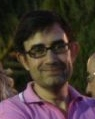
\includegraphics[width = 28 mm]{JJM.jpg},]
\noindent\emph{JJ Merelo} es titular de Universidad en el \'area de
Arquitectura y Tecnolog\'{\i}a de Computadores, y actualmente director de
la Oficina de Software Libre de la UGR. Mantiene un blog desde el a\~no
2002, y lo ha utilizado en clase desde el a\~no 2004; tambi\'en wikis y,
ultimamente, agregadores y otras herramientas TIC. Es partidario del
uso del ordenador conectado en la clase presencial, y lo ha puesto en
pr\'actica, con resultados bastante aceptables.
\end{window}}

\medskip

\small{\begin{window}[0,r,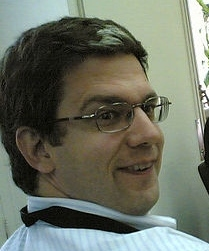
\includegraphics[width = 28 mm]{FTricas1.jpg},]
		\noindent  \emph{Fernando Tricas Garc\'{\i}a} es profesor
		titular de Lenguajes y Sistemas Inform\'aticos del Departamento
		de Inform\'atica e Ingenier\'{\i}a de Sistemas de la Universidad de
		Zaragoza.  Empez\'o a estudiar la blogosfera casi cuando a\'un no
		exist\'{\i}a (all\'a por el a\~no 2002) y a tratar de integrarla en los
		cursos y tareas docentes un poco despu\'es.  Ha impartido
		numerosas charlas relacionadas con el tema de la web 2.0.
		Actualmente (y temporalmente) es Subdirector de Calidad del
		Centro Polit\'ecnico Superior de la Universidad de Zaragoza.  Se
		puede saber m\'as de \'el mirando en su p\'agina web (lo que dice
		que hace y lo que dice que es):
		http://www.cps.unizar.es/~ftricas/ y en su bit\'acora (lo que le
		gusta, o le preocupa, o le llama la atenci\'on)
		http://fernand0.blogalia.com/
\end{window}}

		
\medskip

		\small{\begin{window}[0,r,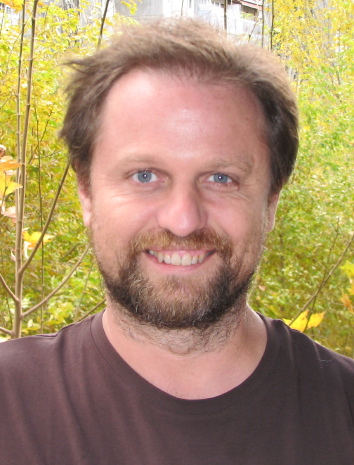
\includegraphics[width = 28
		mm]{Juanjo2.jpg},] \noindent\emph{Juan Jos\'e Escribano Otero}
		es Licenciado en CC Matem\'aticas por la U. Complutense de
		Madrid y doctor por el departamento de CC de la Computaci\'on de
		la U. de Alcal\'a.  Profesor de inform\'atica de la U. Europea de
		Madrid desde 1.993.  Miembro de AENUI desde 2001. Miembro de
		netUEM, grupo de trabajo dedicado a la b\'usqueda de nuevas
		formas de inclusi\'on de nuevas tecnolog\'{\i}as en la docencia
		universitaria desde 2002.
\end{window}}}
%
\noindent   tecnolog\'{\i}a como una herramienta m\'as para
conseguir romper barreras entre el alumno, el profesor y el
aprendizaje, que se sit\'ua como actividad central.

 Es cierto, claro, que los docentes ya utilizaban In\-ter\-net en su tarea,
con diversas aproximaciones, desde el cl\'asico (seg\'un el punto de vista
de hoy en d\'{\i}a) correo electr\'onico a las diversas plataformas web que 
dieron eventualmente lugar a LMS (Learning Management Systems) como
WebCT, Moodle y otros.  Las siglas en este contexto se multiplican:
CMS (Course o Content Management Systems), LCMS (Learning Content
Management System) y uno algo m\'as general, el VLE (Virtual Learning
Environment).  En general, se trataba de herramientas bastante 
completas, que facilitar\'{\i}an la actividad de los profesores y
estudiantes aunque, en nuestra opini\'on, tienen el problema de ser
excesivamente r\'{\i}gidas (es decir, adaptadas a unos flujos de trabajo y
de la informaci\'on preestablecidos y determinados) y adem\'as
concentradas `hacia adentro': el curso, los estudiantes y el profesor,
sin posibilidad (al menos antes del advenimiento de la web 2.0) de
interactuar con el exterior.

Sin embargo, el calificativo 2.0 invoca no s\'olo un cambio en las
herramientas, sino tambi\'en en la actitud: mirando al segundo factor
que influye en la web 2.0, la democratizaci\'on, los estudiantes
deber\'{\i}an poder tomar parte en algunas decisiones sobre el dise\~no de su
aprendizaje y las formas de trabajar que prefieran y las nuevas
herramientas est\'an aqu\'{\i} para ayudarnos en ello.  Ya no se tratar\'{\i}a de
un entorno preparado y preconfigurado por el profesor, sino que el
proceso del aprendizaje podr\'{\i}a venir auxiliado por una serie de
herramientas que `viven' en Internet y que hay (o no) que integrar
para constituir lo que es la informaci\'on sobre el curso y la materia
considerada: es posible que alguien prefiera colaborar utilizando un
wiki, o tal vez mediante GoogleDocs o alguna herramienta similar,
junto con otros que prefieran m\'etodos m\'as tradicionales; no se trata
tanto de centrarnos en la herramienta como de que la diversidad
existente facilite que cada uno encuentre la horma adecuada para su
zapato.

Otra caracter\'{\i}stica b\'asica de lo ``2.0'' que anima a\'un m\'as si cabe el
reto de integrar esta tecnolog\'{\i}a en las ense\~nanzas universitarias es
el concepto de mashup (recombinar).  Dicho vocablo alude a la
posibilidad de construir nuevos servicios 2.0 recogiendo y
recombinando servicios previos.  Ejemplos de mashup hay muchos.
Algunos de los ejemplos m\'as t\'{\i}picos y vistosos se refieren a
recombinaciones derivadas del servicio Google Maps.  Esta posibilidad
de recombinar elementos de un servicio para crear otro, hace que las
posibilidades y servicios aumenten vertiginosamente, provocando una
sensaci\'on de personalizaci\'on casi individual.  El docente y el alumno
pueden, por lo tanto, recoger conocimiento y presentarlo de otra
manera m\'as adaptada a su situaci\'on concreta, tal vez complet\'andolo con
otros servicios, facilitando la actualizaci\'on autom\'atica en cuanto el
servicio original se actualice.

Tampoco hay que perder de vista el contexto en el que se est\'a
trabajando: una universidad espa\~nola con todo lo que ello implica en
los procesos de adquisici\'on y profesionalizaci\'on del profesorado, y un
alumnado que, a pesar de tener conocimientos en nuevas tecnolog\'{\i}as, no
siempre tiene la actitud necesaria para trabajar con ellas; tambi\'en
una universidad en la que la coordinaci\'on docente a veces no llega
mucho m\'as all\'a de evitar que los profesores den clase al mismo tiempo
en la misma aula, y donde hablar de proporcionar ciertas herramientas
a nivel siquiera departamental es muchas veces una utop\'{\i}a.  En este
contexto la experiencia personal adquiere especial relevancia, y es
complicado encontrar evaluaciones pedag\'ogicas externas a la actividad
llevada a cabo por profesores individuales.

Por eso nos proponemos desde esta columna tratar de informar y
descubrir tanto las herramientas que conocemos como las experiencias
interesantes de uso que conozcamos o nos vayan descubriendo: no porque
pensemos que cada herramienta tiene un uso \'unico y concreto sino en la
esperanza de que mostr\'andolas a una comunidad interesada en aprender e
innovar seguramente todos obtengamos mejoras en nuestro proceso de
ense\~nanza y aprendizaje, en nuestra docencia 2.0.

\vspace*{1cm}		

\noindent\rule{90mm}{1pt}

{\small \noindent\copyright 2008 JJ. Merelo, F. Tricas, J.J. Escribano
Otero.  Este art\'{\i}culo es de acceso libre distribuido bajo los t\'erminos
de la Licencia Creative Commons de Atribuci\'on, que permite copiar,
distribuir y comunicar p\'ublicamente la obra en cualquier medio, s\'olido
o electr\'onico, siempre que se acrediten a los autores y fuentes
originales}

\end{multicols}
\end{document}
�
